\documentclass[11pt]{article}
\usepackage{hyperref}
\usepackage{amsthm}
\usepackage{amsmath}
\usepackage{amsfonts}
\usepackage{tikz}
\usepackage{ wasysym }
\usepackage{fancyvrb}
\usetikzlibrary{arrows.meta,positioning}


\newtheorem{example}{Example}


\author{Group 10: Nicholas Jacob}
\title{Homework 8 Advanced Analytics and Metaheuristics}

\begin{document}
\maketitle

\begin{enumerate}
\item Genetic Algorithm
\begin{enumerate}
\item Finalize Code
\begin{enumerate}
\item To create the initial chromosomes, we kept it simple, generating a random number between -500 and 500.  We used the global variable $n$ as the number of dimensions.
\begin{verbatim}
def createChromosome(n):
    x = []   
    for i in range(n):
      x.append(myPRNG.uniform(-500,500))
    return x
\end{verbatim}
\item For mutation, we played with this quite a bit.  Originally we randomly selected an index and the just reseeded it with a random.  This seemed to work but we wanted more control over it so we introduced a new parameter that we could tweak, $mutationFactor$.  We used this to change one of the indicies by a random, $r\in[-1,1]$, with $x[i] = x[i] +r*mutationFactor$.  We could then tweak this factor to get more or less mutation.  We did check that it was inside the interval and if not, randomly reseed.
\begin{verbatim}
def mutate(x):

    if mutationRate > myPRNG.random():
      i = myPRNG.randint(0,n-1)
      x[i] += mutationFactor*myPRNG.uniform(-1,1)
      if (x[i] > 500) or (x[i]<-500):
        x[i] = myPRNG.uniform(-500,500)

    return x
\end{verbatim} 

\item For cross over, we picked on index to swap start the swap.  Everything after that index would be traded between the parents.  This happened with a $crossOverRate$.  Some times just the parents would be returned.
\begin{verbatim}
def crossover(x1,x2):
  p = myPRNG.random()
  if crossOverRate>p:
    z = myPRNG.randint(1,n-1)
    offspring1 = x1[:z] + x2[z:]
    offspring2 = x2[:z] + x1[z:]

  else:
    offspring1 = x1[:]
    offspring2 = x2[:]

  return offspring1, offspring2  #two offspring are returned
\end{verbatim}
\item Elitism was achieved by keeping the best numbering to $eliteSolutions$ from the parent generation.  It was important to resort these as the children were often better.  We also made sure to change it so the minimum was first as desired here.
\begin{verbatim}
def insert(pop,kids):

    newlist = []
    for i in range(eliteSolutions):
      newlist.append(pop[i])
    for kid in kids:
      newlist.append(kid)
    popVals = sorted(newlist, key=lambda newlist: newlist[1], reverse = False)
    return popVals

\end{verbatim}
\item I want to share the code for computing the function.  With $evaluate$ we made sure to utilize the numpy speed in dealing with large dimensional data.
\begin{verbatim}
def evaluate(x):
  x = np.array(x)
  return 418.982887272443*n -sum(x*np.sin(np.sqrt(np.abs(x))))
\end{verbatim}
\end{enumerate}
\item For parameters, I played around with the code a lot.  I noticed for the small dimensional and chromosome, it was important to have higher mutation rate.  I found very good results with the following parameters 
\begin{verbatim}
#number of dimensions in a solution
n = 2

Generations = 300   #number of GA generations

crossOverRate = 0.8  #whether the couple breeds or just continues into next generation
mutationRate = 0.25  #rate at which mutation can occur
eliteSolutions = 10  #number of elite solutions form previous generation that continue on unchanged
mutationFactor = 50 # the largest number by which the mutation can change a random entry
populationSize = 80 #size of GA population
\end{verbatim}

For the higher dimensions, we used 

\begin{verbatim}
#number of dimensions in a solution
n = 200

Generations = 1000   #number of GA generations

crossOverRate = 0.8  #whether the couple breeds or just continues into next generation
mutationRate = 0.25  #rate at which mutation can occur
eliteSolutions = 100  #number of elite solutions form previous generation that continue on unchanged
mutationFactor = 100 # the largest number by which the mutation can change a random entry
populationSize = 1000 #size of GA population
\end{verbatim}
\item 2D
\begin{enumerate}
\item Here is my visualization of 8 chromosomes.  We see some genes splicing and we see some repeats.  It is also possible we see some mutations.

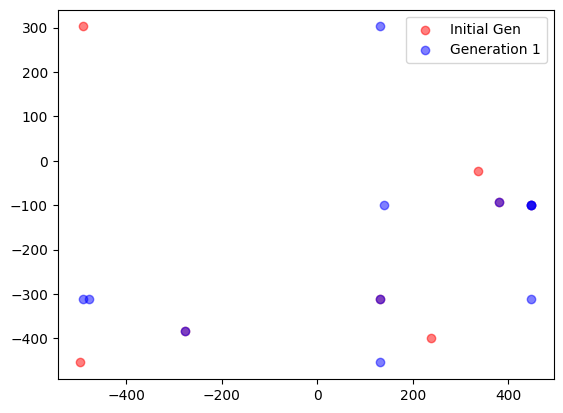
\includegraphics{plot.png}
\item This had Best solution:  [420.9337473832483, 421.0086992961223] as the best solution, accurate to three decimal places, 0.0003559856297670194 
\end{enumerate}
\item This was quite challenging.  At 1000 generations, we were still seeing slight improvements.  This is with an initial population of 1000 and keeping 100 elite solutions.  We saw the value go as low as 18666.  While this is nowhere as good as the 2D solution, we do see many entries with a value near the 420 optimal.  The execution of this code was slow and with the generations not showing much improvement, do not think expanding beyond 1000 generations will improve the result by much.  This problem is hard!
\end{enumerate}
\item Particle Swarm Optimization
\begin{enumerate}
\item Code Basics
\begin{enumerate}
\item Particle Tracking:
\begin{verbatim}
def pbestUpdate(): #update the best lists
  particleUpdate = 0 #how many particles have been updated?
  globalUpdate = 0 #did the global best update
  global pbestestVal, pbestest #get these variables from global environment not local
  for i in range(swarmSize): #iterate through swarm
    if curValue[i]< pbestVal[i]: #is the current better than current best
      pbest[i] = pos[i][:] #since yes, change it up
      pbestVal[i] = curValue[i]
      particleUpdate +=1 #increment the counter
      if curValue[i]<pbestestVal: #since this is better than before, check if it is the new best
        pbestestVal = curValue[i] #since it is, update
        pbestest = pos[i][:]
        globalUpdate +=1
  return particleUpdate, globalUpdate #return counts for stopping criteria
\end{verbatim}
\item Velocity and Position updates
\begin{verbatim}

def velocityUpdate(): #update velocities
  for i in range(swarmSize): #iterate through swarm
    for j in range(dimensions): #iterate through dimensions
      vel[i][j] = w*vel[i][j]+phi1*myPRNG.random()*(pbest[i][j]-pos[i][j])+phi2*myPRNG.random()*(pbestest[j]-pos[i][j]) #follow formula
      if vel[i][j] >maxVelocity: #check if outside of allowed values
        vel[i][j] = maxVelocity #just return max/min allowed
      if vel[i][j] <-1*maxVelocity:
        vel[i][j] = -1*maxVelocity

def positionUpdate():#must be called after velocity update
  for i in range(swarmSize): #iterate through swarm
    for j in range(dimensions): #update all dimensions
      pos[i][j] = pos[i][j] + vel[i][j] #follow basic PSO

      if pos[i][j] > upperBound: #check if outside of feasible
        pos[i][j] = upperBound #if so, put on edge
      if pos[i][j] < lowerBound: #outside feasible?
        pos[i][j] = lowerBound
    curValue[i] = evaluate(pos[i]) #update currentvalue too
\end{verbatim}
\item Limits on particle positions are included in the position update.  I only allow getting on the boundary
\item Limits on velocity are included in velocityUpdate.  Max velocity is a parameter that can be tweaked later.
\end{enumerate}
\item 2D Schwefel
\begin{enumerate}
\item Here is a plot with just positions and velocities.  I don't think those $quiver$ arrows are perfect from $matplotlib$ but they were what was easily available for graphing.

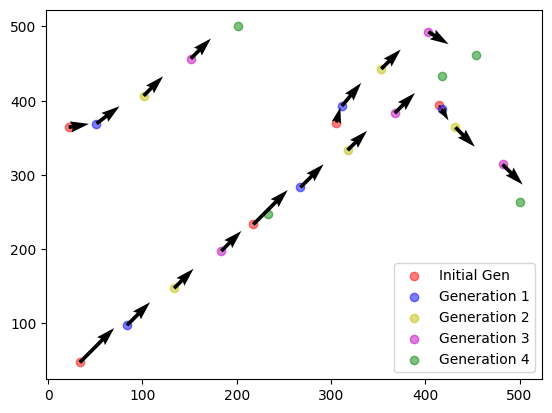
\includegraphics{plot2.png}

\item Here is a plot that includes the global best on each iteration.  Some times the global best was repeated, so that is not reported here.

\includegraphics{plot2Best.png}
\end{enumerate}
\item 200D:  Results are tabulated below.  I really have no theory on what would make this work better.  It felt as though I should be just using random numbers for these parameters as I could not suss out a pattern.  In any case, they are reported here. 

\begin{tabular}{|c|c|c|c|c|c|}\hline
Swarm Size &Time Length & Inertial Weight, $w$ &$\phi_1$ & $\phi_2$& Value\\ \hline
100&1000&1&3&1&44,375\\
10,000&20&1&3&1&71,645\\
1000&200&2&2&2&67,307\\
500&400&0.5&1.5&2.5&48,858\\
750&400&1&1.25&2.75& 67,111\\
100&1000&0&1.25&2.75&57,403
\\ \hline
\end{tabular}
\item Local Best:  I attempted the star topology with all particles being compared to the first of the list.  The modifications to the code base were fairly straight forward.  I needed to make the global best a list and update it by comparing both to the particle at hand and the first particle.  I only make this comparison when I have updated the bestVal already.  The code for doing that is quoted here.  There was also minor changes to the initializers and velocity updates.
\begin{verbatim}
def pbestUpdateLocalStar(): #update the best lists
  particleUpdate = 0 #how many particles have been updated?
  globalUpdate = 0 #did the global best update
  global pbestestVal, pbestest #get these variables from global environment not local
  for i in range(swarmSize): #iterate through swarm
    if curValue[i]< pbestVal[i]: #is the current better than current best
      pbest[i] = pos[i][:] #since yes, change it up
      pbestVal[i] = curValue[i]
      particleUpdate +=1 #increment the counter
      if min(curValue[i],pbestestVal[0])<pbestestVal[i]: #since this is better than before, check if it is a new local best
        if curValue[i] < pbestestVal[i]:
          pbestestVal[i] = curValue[i] #since it is, update
          pbestest[i] = pos[i][:]
          globalUpdate +=1
        else:
          pbestestVal[i] = pbestestVal[0] #since it is, update
          pbestest[i] = pbestest[0][:]
          globalUpdate +=1

  return particleUpdate, globalUpdate #return counts for stopping criteria

\end{verbatim}
\item Test with Local:  Lastly I repeat the code a bunch of times and add to the table now with the local star topology.  I attempted to reuse the values from before so this table looks a lot like the one above.

\begin{tabular}{|c|c|c|c|c|c|}\hline
Swarm Size &Time Length & Inertial Weight, $w$ &$\phi_1$ & $\phi_2$& Value\\ \hline
100&1000&1&3&1&68,874\\
10,000&20&1&3&1&72,464\\
1000&200&2&2&2&73,569\\
50&400&0.5&1.5&2.5&78,151\\
750&400&1&1.25&2.75& 69,092\\
100&1000&0&1.25&2.75& 77,421
\\ \hline
\end{tabular}

Overall, I do not see marked improvement based on the star topology.  Seems like leaderless swarms are better, since this one clearly has a leader and you are always checking only if you did better than them.  Also making the inertial weight 0 was a bad choice as it did not explore...  
\end{enumerate}
\end{enumerate}
Overall I much preferred the genetic algorithm.  It felt more natural for this problem but perchance I just didn't play around enough to get this one tweaked to work well...


\end{document}
